We begin by performing a very simple screening of the available potentials using 0~K potential energy calculations.
The energy for the relevant ideal Fe-Al phases is shown in Fig.~\ref{fig:0K_phases}.
Here we can already see that the potentials of Farkas \etal~\cite{farkas2020model} and Jelinek \etal~\cite{jelinek2012modified} both fail to provide clear BCC stability.
This is not shocking as these were both designed for high-entropy alloys, and the former is explicitly targeted towards the FCC phase.
Nonetheless, for the rest of our investigation we can safely focus on the EAM potential of Mendelev \etal~\cite{mendelev2005effect} and the more recent MEAM potential of Lee and Lee \etal~\cite{lee2010modified}.
%
\begin{figure}[h]
    \centering
    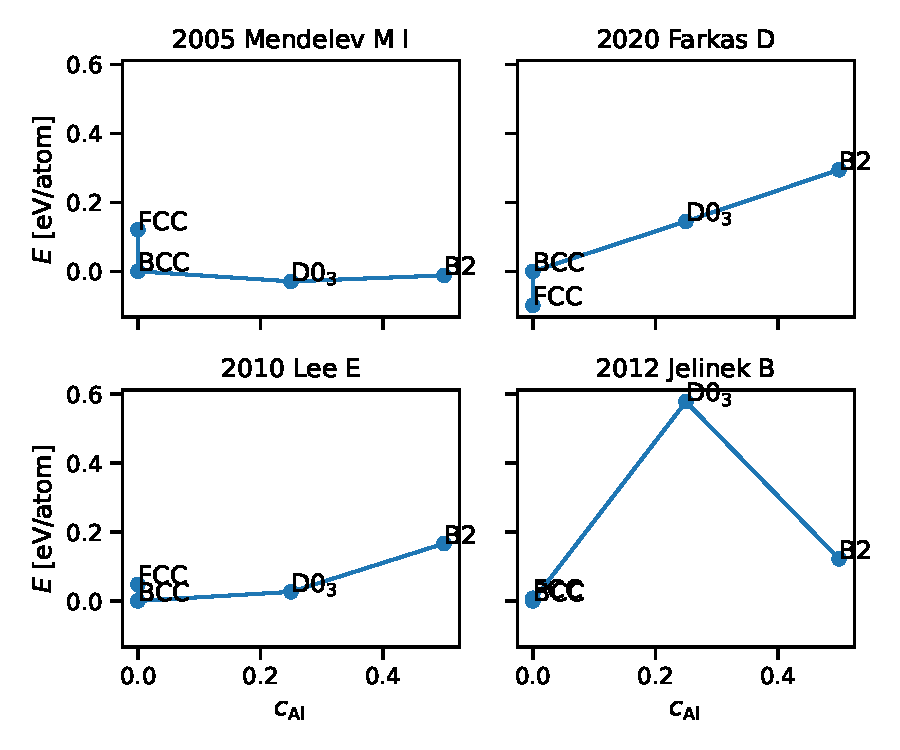
\includegraphics[width=\textwidth]{figures/zerok_phases}
    \caption{0K potential energy/atom for each of the relevant Fe-Al phases up to 50\% Al for several empirical potentials~\cite{mendelev2005effect, lee2010modified, jelinek2012modified, farkas2020model}.}
    \label{fig:0K_phases}
\end{figure}

In addition to being BCC stable, we know that the potentials should be dominated by a solid solution at 18\% Al, and that at higher concentrations the \DOTHREE phase should also be energetically competitive.
To this end, the expanded diagram in Fig.~\ref{fig:expanded_0K_phases} to include the random solid solution energy at Al concentrations up to the nominal \DOTHREE concentration.
At each concentration ten different random configurations of 432 atoms ($6\times6\times6$ BCC units) we relaxed at zero pressure, and the final energy averaged over.
The error bars for the solid solution shows the 95\% confidence interval from the sampling (i.e. roughly double the standard deviation).
During our exploration we discovered that the Mendelev potential actually shows a strong preference for alternative ordered structures with columnar and planar Al.
We included these configurations at different Al concentration by varying their inter-columnar or inter-planar spacing.
Representatives of all of these are visualized in Fig.~\ref{fig:structures}.
%
\begin{figure}[h]
    \centering
    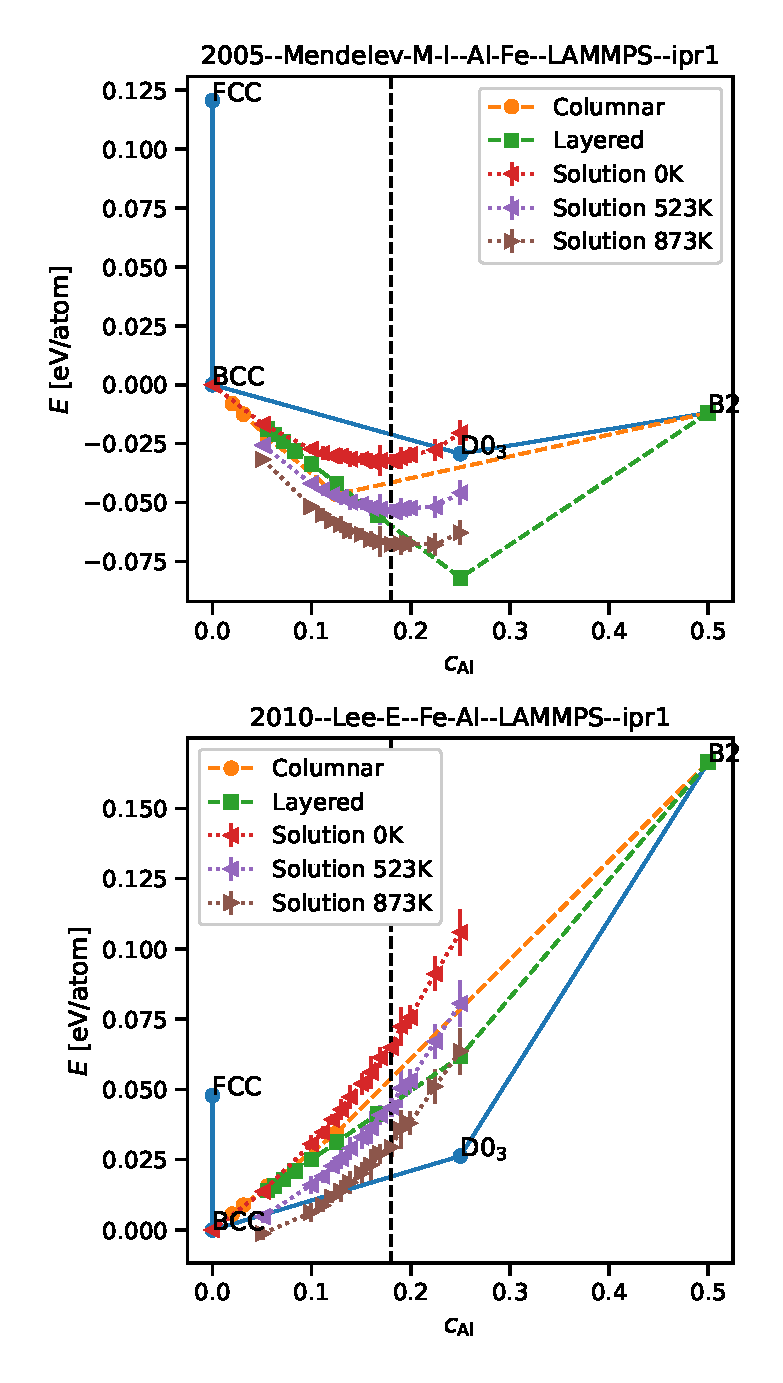
\includegraphics[width=\textwidth,height=0.75\textheight,keepaspectratio]{figures/expanded_0K_phases}
    \caption{0K potential energy/atom for the regular phases, but also columnar Al (orange circles), planar Al (green squares), and random solid solution including configurational entropy at three temperatures, 0~K, 523~K, and 873~K (triangles red, purple, and brown, respectively) with error bars showing a 95\% confidence interval for the average solution energy.}
    \label{fig:expanded_0K_phases}
\end{figure}
%
\begin{figure}[h]
    \centering
    \includegraphics[width=\textwidth,height=\textheight,keepaspectratio]{figures/structures}
    \caption{Representative visualizations of the structures for (a) FCC, (b) BCC (with 18\% Al), (c) \DOTHREE, (d) \BTWO, (e) the columnar structure, and (f) the planar structure. Al is shown small and grey while Fe is larger and red.}
    \label{fig:structures}
\end{figure}

In addition to the 0~K potential energy, for the BCC solid solution, the ideal entropy of mixing was included at both the experimental annealing temperatures.
This demonstrates the increasing benefit to the \emph{free} energy for the system to occupy a disordered state.
In principle the entropy of mixing is also relevant for the other phases -- even our SRO clusters may contain chemical antisites and do not need to \emph{perfectly} conform to the reference ordering -- but at this stage they are omitted, as is vibrational entropy for all phases.
Even with these simplifications, we can already draw important conclusions: first, the Mendelev potential will never display \DOTHREE SRO at 18\% Al, and indeed even at the nominal \DOTHREE concentration of 25\% Al it is \emph{still} not the preferable state for this potential -- by constructing a parallel tangent line between the minima of the phases, we can expect the system is likely to form either a composition of solid solution and the layered structure, or simply form into ordered layers.
The potential energy of this layered structure sits so far below the \DOTHREE phase that we should never expect to see \DOTHREE form in any significant fraction.
Second, \BTWO formation is similarly unlikely at the nominal alloy composition, although the preference for planar and columnar Al configurations can be interpreted as colmnar or planar \BTWO (which is not what was found experimentally, where \BTWO SRO clusters are generally spherical).
The third key observation is that for the Lee potential a similar Gibbs-tie-line analysis shows that decomposition into solid solution and \DOTHREE \emph{is} possible, but may only occur at higher temperatures than we expect from experiment -- at the lower temperature of 523 K we can also expect a decomposition into BCC and \DOTHREE, but with almost no Al in the BCC solution.
I.e. this potential seems to have an unphysically low solubility of Al in bulk BCC Fe.
Finally, for the Lee potential we also do not expect any \BTWO SRO.

Next, to allow the full interplay and competition of all factors including vibrational entropy, we perform full MCMD calculations using the variance constrained approach~\cite{sadigh2012calculation, sadigh2012scalable} (with a relatively strict constraint $\kappa = 1e4$) to maintain the Al concentration very close to the nominal experimental value of 18\%.
Estimating the chemical potential, $\Delta \mu$ from the change in 0~K potential energies of the most favourable phases -- BCC and \DOTHREE (layered Al) for the Lee (Mendelev) potential -- gives $|\Delta \mu| < 0.1~\mathrm{eV}$ ($<0.3~\mathrm{eV}$) for the Lee (Mendelev) potential.
As seen by the inclusion of just configurational entropy to the solid solution phase, this is very likely to be an upper bound to the true chemical potential, as point defects in the secondary phase would lower its free energy and further reduce the slope of any Gibbs tie line.
Since the application of the variance constraint means that the chemical potential does not ultimately influence the nature of the results obtained but only the computational efficiency (i.e. number of MC steps required) we safely approximate $\Delta \mu = 0 $ for both potentials.
With a 1 fs timestep for integration, these simulations ran for 100 ps each, with MC trial swaps for 10\% of the atoms every 0.1 ps.
Although smaller than the experimental dimensions, the simulation cells were of the same order of magnitude: $4\times4\times4$ nanometer periodic cubes (5488 atoms) in a periodic domain.
We can get a quick sense of whether the system has converged to the desired chemical ordering by examining the equilibration of the potential energy as a function of time/MC steps.
This is shown in Fig.~\ref{fig:energy_conv} where we see that all systems except for the Lee potential at 523~K have converged to fluctuate around the average energy of the back half of the simulation.
In contrast, the Lee potential at 523 K still shows a clear trend of decreasing energy, indicating that it has not reached its equilibrium configuration at all.
This slow convergence can be understood in light of Fig.~\ref{fig:expanded_0K_phases}, since at this temperature we are most likely in a miscibility gap between very low concentration solid solution and \DOTHREE;
starting from an initial configuration of random solid solution with 18\% Al, the system is trying to decompose into pure \DOTHREE and BCC with almost no Al, a process which requires many, many MC swaps.
%
\begin{figure}[h]
    \centering
    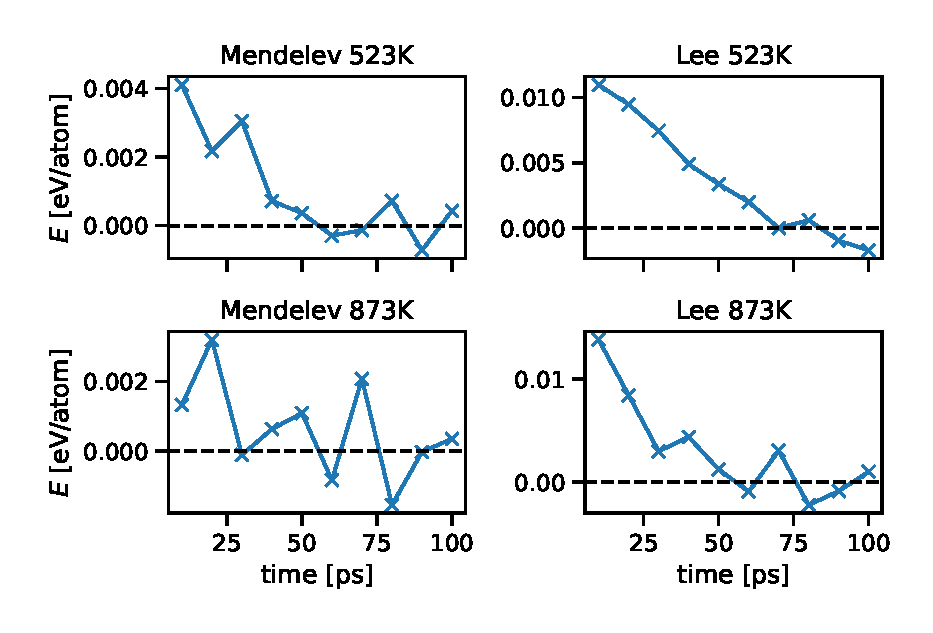
\includegraphics[width=\textwidth]{figures/energy_conv}
    \caption{Potential energy convergence as a function of time (and thus MC swaps) for Mendelev~\cite{mendelev2005effect} and Lee~\cite{lee2010modified} potentials at high and lower temperture. Dashed line shows the average energy for the last five frames.}
    \label{fig:energy_conv}
\end{figure}

Unlike the experimental APT data, we have full access to the species and position of each atom in our computational sample.
Thus, to analyze SRO into the specific \DOTHREE and \BTWO configurations observed in experiment, we can directly check whether each atom has a local environment that matches the target phase.
We do this by constructing the topology of our system considering all 14 first- and second-nearest neighbours (NN) to be ``connected'', and comparing the species of the atom under question as well as all of its neighbours to one of six references: two from the \BTWO pattern with Al occupying either simple-cubic sublattice, and four symmetry-equivalent organizations of \DOTHREE.
Using a breadth-first-search, for each of the six reference patterns we construct all matching clusters.

The size and number of clusters found is then dependent on how strictly we demand that the test environment match the reference environment;
if we very strictly insist that each atom in a cluster be surrounded by \emph{exactly} the reference cluster, it is more difficult to find clusters beyond a few atoms in size given the entropic favourability of point defects in the secondary phase;
however, at the opposite extreme, if we are too relaxed in our condition and allow atoms with only a few neighbours matching the reference to count towards a cluster, then the entire system is consumed with one erroneous ``cluster''.
To overcome this we must make reference to the same clustering algorithm applied to the truly random solid solution used as input to the MCMD simulations, and consider the \emph{changes} in the cluster distribution after the sample has been allowed to equilibrate its chemical ordering.
We found that a threshold value of 13 of the 14 NN gives us gives good resolution for contrasting the random sample -- where clusters may occur by pure chance -- and the MCMD annealed samples -- where clusters may still occur by pure chance, but also may form due to a driving force for SRO.
The interested reader can examine the \code{github} repository~\cite{feal} for more detail.

The resulting histograms for identified clusters -- ignoring \emph{single atom} ``clusters'' and binning by ten atoms at a time -- can be seen in Figs.~\ref{fig:mendelev_hist} and \ref{fig:lee_hist} for the Mendelev and Lee potentials, respectively.
The Mendelev potential shows a very mild decrease in \DOTHREE clusters, suggesting that the small random clusters may have some small driving force to group together into fewer, very slightly larger clusters.
For \BTWO the opposite effect is seen, but it is clear from examining the total number of clusters that this is trivial.
At neither temperature and for neither reference phase does the Mendelev potential exhibit SRO to either of the relevant phases.

Meanwhile, the Lee potential shows a similar non-result for \BTWO ordering, but we observe a distinct trend for SRO of \DOTHREE clusters, especially at the higher temperature.
At 523 K we see one medium sized cluster (about 50 atoms) and ten small clusters in the 10-20 atom range,
but this calculation was poorly converged.
At 873 K the calculation was well converged and here we see four large clusters (>100 atoms, where the binning is truncated), as well as a collection of medium sized clusters, and some small clusters.
Note that this histogram is truncated at a size of 100, so the four counts at the largest size are actually all different sizes, each some hundreds of atoms.

By referring back to Fig.~\ref{fig:expanded_0K_phases}, we can see that we expect to be in the miscibility gap between the solid solution and \DOTHREE phases.
So, at 873 K where we see the formation of a whole distribution of clusters, are we really at a thermodynamic equilibrium or is this merely a transient state on the path to perfect phase separation?
Even though we are inside a miscibility gap, and ignoring unlikely scenarios like a negative solid solution/\DOTHREE interface energy, there is still a clear explanation for why we may observe SRO instead of \emph{only} decomposition: while the system still wants to form \DOTHREE, there at higher temperatures there is an increased entropic benefit to allowing this \DOTHREE to occur in many small clusters spread throughout the system instead of by full phase separation.
In the classic image of a TTT diagram, we may be up above the nose, where the formation of a precipitate above the critical size for Ostwald ripening (i.e. completely stable against decomposition) becomes exceedingly unlikely -- or at least takes a very long time.
Since the MCMD infrastructure is not well-optimized for MEAM potentials like the Lee potential, simply running much longer is not a desirable solution.

%
\begin{figure}[h]
    \centering
    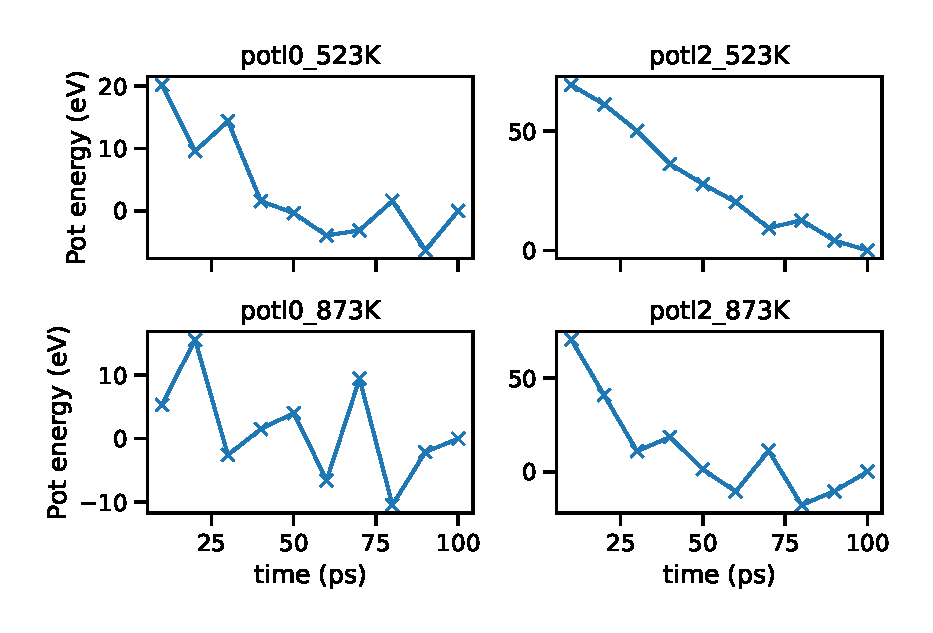
\includegraphics[width=\textwidth]{figures/mendelev_hist_thresh13}
    \caption{Cluster counts (ignoring single atom ``clusters'') for the Mendelev potential before (blue) and after (orange) MCMD equilibration from a random mixture, shown for \DOTHREE and \BTWO reference phases at two different temperatures.}
    \label{fig:mendelev_hist}
\end{figure}
%
\begin{figure}[h]
    \centering
    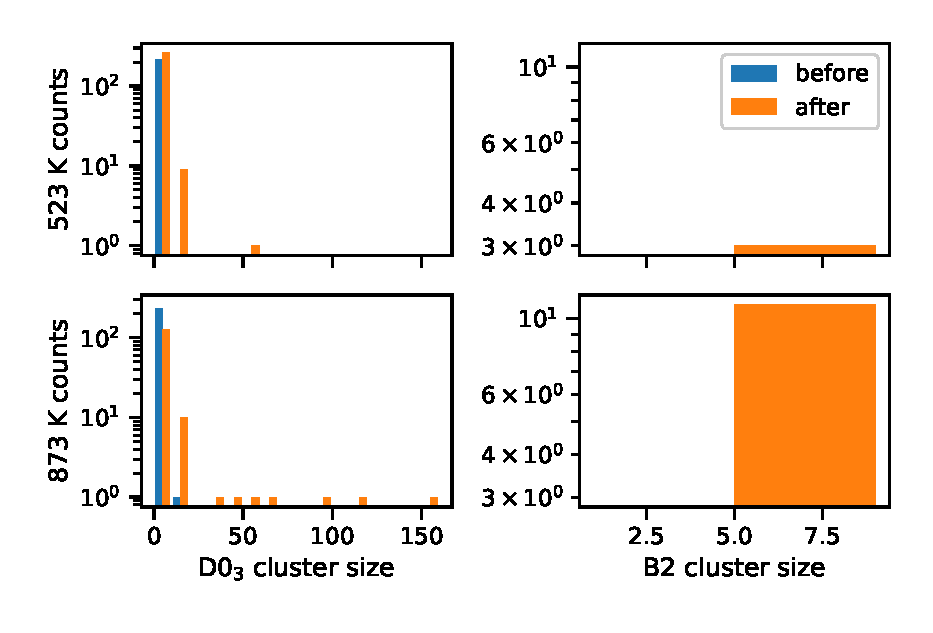
\includegraphics[width=\textwidth]{figures/lee_hist_thresh13}
    \caption{Cluster counts (ignoring single atom ``clusters'') for the Lee potential before (blue) and after (orange) MCMD equilibration from a random mixture, shown for \DOTHREE and \BTWO reference phases at two different temperatures. Binning is truncated at 100, so larger clusters are all lumped into the final bin shown.}
    \label{fig:lee_hist}
\end{figure}

One alternative approach is to change our MCMD initial conditions by \emph{starting} from perfect phase separation instead of starting from random solution.
In this case, at high temperature we expect this perfect \DOTHREE precipitate to decompose to bring the solid solution equilibrium value and then to still see the formation of new \DOTHREE SRO clusters forming in the BCC domain.
At the lower temperature, in contrast, our earlier calculations with 0~K energy and configurational entropy indicate that the equilibrium concentration of Al in the BCC phase will be extremely low.
Under these conditions it should be very difficult for enough Al to come together for short lived SRO clusters, and we expect little to no decomposition of the initial monolithic precipitate.

Here, we have used a (roughly) spherical \DOTHREE coherent precipitate in the pure-Fe BCC bulk, with the size of the precipitate tuned so that the Al concentration is still 18\%.
Results of the cluster analysis through time can be see in Fig.~\ref{fig:lee_dissolution} at both temperatures -- the single largest cluster of more than 4000 atoms is not shown.
Indeed, at the lower temperature there is zero indication of any dissolution of the initial precipitate.
Some of the intermediate steps show a change in cluster counts for the 2-10 atom range, which may occur as Al atoms swap into the BCC bulk for a transient existence as a point defect, but no other clusters form and survive and the final Al concentration in the BCC is still zero.
The remaining small clusters occur because some Fe atoms are able to register as having a \DOTHREE-like environment while being perfectly surrounded by other Fe atoms.
On the other hand, at 873 K, we see clear evidence that the precipitate is dissolving: there are dozens of small clusters (2-10 atoms) and one or two slightly larger clusters (20-30 atoms) throughout the simulation, and the final Al concentration in the BCC bulk is 4\%.
Just as the cold simulation starting from the random solution did not fully equilibrate, neither does the hot simulation starting from full phase decomposition, but the qualitative trend is completely consistent with our earlier observation of SRO in the high temperature-random start MCMD calculation.

\begin{figure}[h]
    \centering
    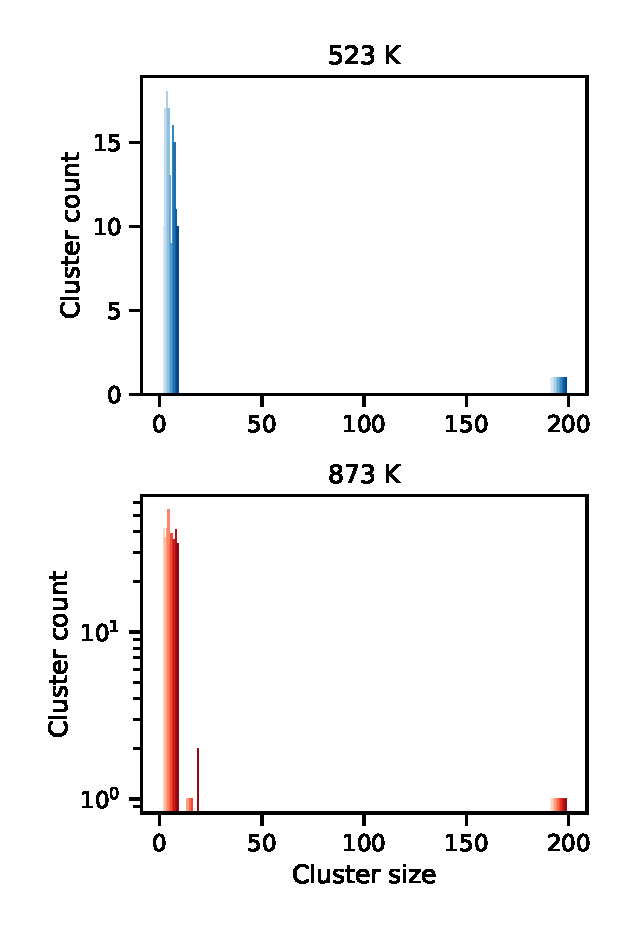
\includegraphics[width=\textwidth,height=0.75\textheight,keepaspectratio]{figures/decomposing_clusters}
    \caption{Identified \DOTHREE clusters evolving with the Lee potential from an initial state of full BCC-\DOTHREE phase separation. Results for (a) 523 K and (b) 873 K show evolution through time with darker bars being later in the simulation.}
    \label{fig:lee_dissolution}
\end{figure}

If this entropically-driven perspective is correct, we should also see that the observed SRO clusters are not infinitely long lived, but eventually dissolve only to reform somewhere else.
To study this, we can look at what fraction of sites identified as part of a \DOTHREE cluster are new, i.e. were not identified as \DOTHREE sites in the last snapshot of the system's evolution.
This is shown in Fig.~\ref{fig:turnover} at both low and high temperature for the Lee potential starting from random solid solution.
Due to the large amount of MD time (10 ps) and large number of trial MC swaps (10\% of the system 100 times), we can expect the sequential snapshots to be quite well decorrelated.

By studying the system energy as a function of time back in Fig.~\ref{fig:energy_conv} we know that the 523 K simulation is not well converged.
With the additional data here we see that less than 20\% of the \DOTHREE sites in each snapshot are new, and indeed this roughly corresponds to total number of additional sites as the system continues to phase decompose!
So at this low temperature we effectively have the formation and ripening of clusters.
In contrast, although there is still some weak upwards trend in the total number of \DOTHREE sites, at 873 K we see that the phase transformation has more or less stabilized for the last five snapshots.
In this near-equilibium regime, we see that full \emph{half} of the atoms participating in a \DOTHREE cluster are not preserved from snapshot to snapshot.
This is completely consistent with our picture of the ``rolling boil'' of SRO precipitates forming, dissolving, and reforming at this high temperature.

\begin{figure}[h]
    \centering
    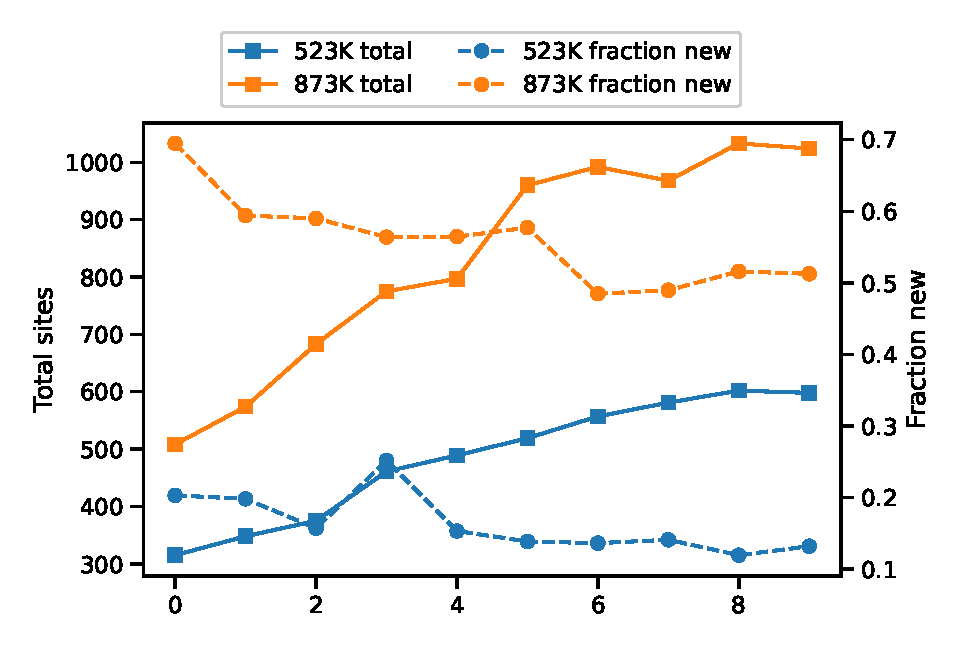
\includegraphics[width=\textwidth,height=0.75\textheight,keepaspectratio]{figures/cluster_turnover}
    \caption{Total number of \DOTHREE sites identified at each frame (solid) (i.e. 10 ps MD time and 100 iterations of performing MC trials on 10\% of the system) and the fraction of sites which were \emph{not} in clusters in the last frame (dashed). Results shown for 523 K (blue circles) and 873 K (orange squares).}
    \label{fig:turnover}
\end{figure}

As a bit of an aside, we can also test whether Fig.~\ref{fig:expanded_0K_phases} makes accurate predictions for the Mendelev potential.
Testing for columnar or planar precipitates is harder, because we do not have the same easy reference system to compare to.
However, both these shapes can be thought of as a very particularly arranged \BTWO precipitate.
By weakening our clustering criterion to 11 out of 14 NN and examining some of the larger \BTWO clusters identified, we can indeed locate the formation of small plate-like precipitates which support the planar phase, shown in Fig.~\ref{fig:mendelev_structure}(a) where one of the larger clusters is plotted for the equilibrated system at 523~K.
Partial columns of Al are also clearly visible in the full structure, also shown in Fig.~\ref{fig:mendelev_structure}(b).
As with the other structure plots, the atoms are always mapped back to their lattice positions, although their true atomic positions of the snapshot are disorderly as they are the output of an MD trajectory.
%
\begin{figure}[h]
    \centering
    \includegraphics[width=\textwidth,height=0.75\textheight,keepaspectratio]{figures/equilibrated_mendelev_523}
    \caption{(a) one of the larger \BTWO clusters constructed with a more relaxed clustering condition of 11 NN and (b) the complete structure from the end of the MCMD equilibration with the Mendelev potential at 523~K.}
    \label{fig:mendelev_structure}
\end{figure}